\documentclass[DIN, pagenumber=false, fontsize=11pt, parskip=half]{scrartcl}

%\usepackage{ngerman}
\usepackage[spanish]{babel}
\selectlanguage{spanish}
\usepackage[utf8]{inputenc}
\usepackage[T1]{fontenc}
\usepackage{textcomp}
\usepackage{ amssymb }
\usepackage{float}
\usepackage{graphicx}

%\usepackage[spanish]{babel}

% for matlab code
% bw = blackwhite - optimized for print, otherwise source is colored
\usepackage[framed,numbered,bw]{mcode}

% for other code
%\usepackage{listings}

\setlength{\parindent}{0em}

% set section in CM
\setkomafont{section}{\normalfont\bfseries\Large}

\newcommand{\mytitle}[1]{{\noindent\Large\textbf{#1}}}
\newcommand{\mysection}[1]{\textbf{\section*{#1}}}
\newcommand{\mysubsection}[2]{\romannumeral #1) #2}
\usepackage{color}







\usepackage[utf8]{inputenc}

\usepackage[margin=1in]{geometry}
\usepackage{amsmath,amssymb}
\usepackage{multicol}

\newcommand{\class}{Relatividad General}
\newcommand{\term}{2017 -2}
\newcommand{\examnum}{Tercer Parcial}
\newcommand{\examdate}{29/11/2017}
%\newcommand{\timelimit}{60 Minutes}







%===================================
\begin{document}




\noindent
\begin{tabular*}{\textwidth}{l @{\extracolsep{\fill}} r @{\extracolsep{6pt}} l}
\textbf{\class} & \textbf{Name:} & Johan S. Méndez\\
\textbf{\term} &&\\
\textbf{\examnum} &&\\
\textbf{\examdate} &&\\
\textbf{} & \textbf{Profesor} & Alexis Larrñaga
\end{tabular*}\\
\rule[2ex]{\textwidth}{2pt}



La métrica a estudiar será

\begin{equation}
\label{metrica}
    ds^{2} = \left(1-\frac{2M}{r}\right)dt^{2}+\left(1-\frac{2M}{r}\right)^{-1}dr^{2} +r^{2}\left(1-\frac{Q^{2}}{Mr}\right)\left(d\theta^{2}+\sin^{2}\theta d\phi^{2}\right)
\end{equation}

Lo que se quiere estudiar en particular para esta métrica es:

\begin{itemize}
    \item Potencial efectivo 
    \item Estudiar el tipo de trayectorias posibles a través de consideraciones en el el potencial efectivo
    \item Encontrar ecuación de la trayectoria
\end{itemize}

En primer lugar se plantea el Lagrangiano a partir de la consideración de la métrica ( \ref{metrica})

\begin{equation*}
    \mathcal{L} = \left(1-\frac{2M}{r}\right)\left(\frac{dt}{d\tau}\right)^{2}+\left(1-\frac{2M}{r}\right)^{-1}\left(\frac{dr}{d\tau}\right)^{2} +r^{2}\left(1-\frac{Q^{2}}{Mr}\right)\left(\left(\frac{d\theta}{d\tau}\right)^{2}+\sin^{2}\theta \left(\frac{d\phi}{d\tau}\right)^{2}\right)
\end{equation*}

Entonces se encuentran las ecuaciones de movimiento. Se evidencia que el Lagrangiano no depende explícitamente del tiempo, entonces se utilizan las ecuaciones de Euler Lagrange, en primer lugar

\begin{eqnarray*}
    \frac{\partial}{\partial \tau}\left(\frac{\partial\mathcal{L}}{\partial \dot{t}} \right) = \frac{\partial\mathcal{L}}{\partial t} &=& 0 \\
    \frac{\partial }{\partial \tau}\left(-2\left(1-\frac{2M}{r}\right)\dot{t}\right) &=& 0\\
    \left(1-\frac{2M}{r}\right)\dot{t} &=& E\quad(\text{cte}) \\
\end{eqnarray*}

Por tanto, la energía es una constante de movimiento, se tiene por lo tanto 

\begin{eqnarray}
\label{energia}
    \dot{t}^{2} = \frac{E}{(1-2M/r)^{2}}
\end{eqnarray}
    
Para seguir desarrollando el problema se estudia la ecuación de movimiento de la variable $\theta$

\begin{eqnarray*}
    \frac{\partial}{\partial \tau}\left(\frac{\partial\mathcal{L}}{\partial \dot{\theta}} \right) &=& \frac{\partial\mathcal{L}}{\partial \theta}  \\
    \frac{\partial }{\partial \tau}\left(2r^{2}\left(1-\frac{Q^{2}}{Mr}\right)\dot{\theta}\right) &=& 2r^{2}\sin\theta\cos\theta\dot{\phi}^{2}\\
    \frac{\partial }{\partial \tau}\left(r^{2}\left(1-\frac{Q^{2}}{Mr}\right)\dot{\theta}\right) &=& r^{2}\sin\theta\cos\theta\dot{\phi}^{2}
\end{eqnarray*}

Sí se impone una condición inicial $\theta(0) = \pi/2$ y $\dot{\theta} 0$, se tiene que el cuerpo se está moviendo inicialmente en el plano ecuatorial. Por esta razón siempre se puede elegir los ejes coordenados con el eje normal z al plano de movimiento, entonces se asume que $\theta = \pi/2$

Ahora se estudia la variable $\phi$, como no se evidencia explicitamente en el Lagrangiano debe conservarse el momento angular 

\begin{eqnarray*}
    \frac{\partial}{\partial \tau}\left(\frac{\partial\mathcal{L}}{\partial \dot{\phi}} \right) &=& \frac{\partial\mathcal{L}}{\partial \phi} = 0   \\
    \frac{\partial }{\partial \tau}\left(2r^{2}\left(1-\frac{Q^{2}}{Mr}\right)\sin^{2}\theta\dot{\phi}\right) &=& 0 \\
    \frac{\partial }{\partial \tau}\left(r^{2}\left(1-\frac{Q^{2}}{Mr}\right)\sin^{2}\theta\dot{\phi}\right) &=& l \quad (\text{cte})
\end{eqnarray*}

Entonces se tiene

\begin{equation}
\label{momento_angular}
    \dot{\phi}^{2} = \frac{l^{2}}{r^{4}(1-Q^{2}/Mr)^{2}}
\end{equation}

Entonces el lagraniano toma la siguiente forma, utilizando (\ref{momento_angular}), (\ref{energia}).

\begin{eqnarray*}
    \mathcal{L} = -\left(1-\frac{2M}{r}\right)^{-1}E + \left(1-\frac{2M}{r}\right)^{-1}\dot{r}^{2} + \left(1-\frac{Q^{2}}{Mr}\right)^{-1}\frac{l^{2}}{r^{2}}
\end{eqnarray*}

Del lagrangiano se tienen las siguientes condiciones 

\begin{eqnarray}
\label{delta}
     \mathcal{L} =  -c^{2}\left \{ \begin{matrix} 1 & \mbox{si son partículas con masa} 
\\ 0 & \mbox{si son particulas sin masa}\end{matrix}\right. = -c^{2}\delta 
\end{eqnarray}

Entonces se tiene que si se despeja la energía se llega a 

\begin{eqnarray}
\label{Energia}
    E = \dot{r}^{2}+\left(1-\frac{2M}{r}\right)\left[\delta +\left(1-\frac{Q^{2}}{Mr}\right)^{-1}\frac{l^{2}}{r^{2}}\right]
\end{eqnarray}

Desde aca se obtiene el potencial efectivo 

\begin{equation}
    V_{eff} = \left(1-\frac{2M}{r}\right)\left[\delta +\left(1-\frac{Q^{2}}{Mr}\right)^{-1}\frac{l^{2}}{r^{2}}\right]
\end{equation}

A continuación el potencial efectivo para partículas 

\begin{figure}[H]
\centerline{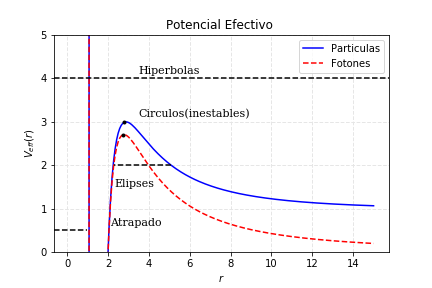
\includegraphics[scale =0.8]{Particulas.png}}
\caption{Resultado de graficar el potencial efectivo en función de $r$, está dada con los siguientes parámetros. $M = 1$, $Q = 1$, $l = 6.9$}
    \label{2}
\end{figure}

Para poder deducir la ecuación de la trayectoria ($r = r(\phi)$) se hace el acostumbrado cambio de variable $u = 1/r$, por tanto 

\begin{eqnarray*}
    \dot{r} = \frac{dr}{d\phi}\frac{d\phi}{d\tau} \rightarrow \dot{r} = \frac{dr}{d\phi}\dot{\phi}\rightarrow\frac{dr}{d\phi} = \frac{\dot{r}}{\dot{\phi}} \rightarrow \dot{r}^{2} = \dot{\phi}^{2}\frac{dr}{d\phi}\\
    \dot{r}^{2} = \frac{l^{2}}{r^{4}(1-Q^{2}/Mr)^{2}}\frac{dr}{d\phi}, \qquad \frac{dr}{d\phi} = \frac{d(1/u)}{d\phi} = -\frac{1}{u^{2}}\frac{du}{d\phi}
\end{eqnarray*}

Luego de esto se puede reemplazar en (\ref{Energia}) y obtener

\begin{eqnarray*}
    E = \frac{Ml^{2}}{M-Q^{2}u}\left(\frac{du}{d\phi}\right)^{2}+\left[(1-2Mu)\delta +\frac{Ml^{2}u^{2}}{M-Q^{2}u}-\frac{2M^{2}l^{2}u^{3}}{M-Q^{2}u}\right]
\end{eqnarray*}

Pongamos por facilidad en la notación $du/d\phi = u_{\phi}$

\begin{eqnarray*}
    E = \frac{Ml^{2}}{M-Q^{2}u}u_{\phi}^{2}+\left[(1-2Mu)\delta +\frac{Ml^{2}u^{2}}{M-Q^{2}u}-\frac{2M^{2}l^{2}u^{3}}{M-Q^{2}u}\right]
\end{eqnarray*}

Se consigue la forma de la ecuación diferencial con algunos pasos algebráicos

\begin{eqnarray*}
    u_{\phi}^{2} + \left(1+\frac{2Q^{2}\delta}{l^{2}}\right)u^{2} = \frac{E-\delta}{l^{2}}+\left(\frac{(2M^{2}+Q^{2})\delta}{Ml^{2}}-\frac{Q^{2}E}{Ml^{2}}\right)u + 2Mu^{3}
\end{eqnarray*}

Derivando respecto de $\phi$ se obtiene

\begin{eqnarray*}
    2u_{\phi}u_{\phi\phi} + 2\left(1+\frac{2Q^{2}\delta}{l^{2}}\right)uu_{\phi} = \left(\frac{(2M^{2}+Q^{2})\delta}{Ml^{2}}-\frac{Q^{2}E}{Ml^{2}}\right)u_{\phi} + 6Mu^{2}u_{\phi}\\
    u_{\phi}\left(u_{\phi\phi} + \left(1+\frac{2Q^{2}\delta}{l^{2}}\right)u- \left(\frac{(2M^{2}+Q^{2})\delta}{2Ml^{2}}-\frac{Q^{2}E}{2Ml^{2}}\right) -3Mu^{2}\right) = 0
\end{eqnarray*}

Desde acá se tiene que $u_{\phi} = 0$ lo que nos lleva a $dr/d\phi = 0 \longrightarrow r =$ cte, es decir que las trayectorias podrían tomar órbitas circulares, para las otras posibilidades se debe resolver la ecuación diferencial

\begin{eqnarray}
    u_{\phi\phi} -3Mu^{2} + \left(1+\frac{2Q^{2}\delta}{l^{2}}\right)u =  \left(\frac{(2M^{2}+Q^{2})\delta}{2Ml^{2}}-\frac{Q^{2}E}{2Ml^{2}}\right)  
\end{eqnarray}

Se hace entonces los dos posibles casos, dada la definición de $\delta$ (\ref{delta})

si $\delta = 0$

\begin{eqnarray}
    u_{\phi\phi} -3Mu^{2} + u =  -\frac{Q^{2}E}{2Ml^{2}} 
\end{eqnarray}

Ahora si $\delta = 1$

\begin{eqnarray}
    u_{\phi\phi} -3Mu^{2} + \left(1+\frac{2Q^{2}}{l^{2}}\right)u =  \left(\frac{(2M^{2}+Q^{2})}{2Ml^{2}}-\frac{Q^{2}E}{2Ml^{2}}\right)  
\end{eqnarray}

\end{document}



